%% ****** Start of file rsitemplate.tex ****** %
%%
%%   This file has been edited from the original source file.
%%	 The original file is part of the revtex4-1 package indicated below.
%%   Version 4.1 of 9 October 2009.
%%
%
% This is a template for producing documents for use with 
% the REVTEX 4.1 document class and the RSI substyle.
% 
% Copy this file to another name and then work on that file.
% That way, you always have this original template file to use.
\documentclass[aip,rsi,reprint]{revtex4-1} % for checking your page length
%\documentclass[aip,rsi,reprint,graphicx,draft]{revtex4-1} % for checking your page length
%\\documentclass[aip,rsi,preprint,graphicx]{revtex4-1} % for review purposes

\usepackage{siunitx}
\DeclareSIUnit{\sqrthz}{\ensuremath{\sqrt{\text{\hertz}}}}

\usepackage{amsmath}
\usepackage{amsfonts}

\usepackage{graphicx}
\usepackage{dcolumn}
\usepackage{multirow}
%\usepackage{caption}
%\usepackage{subcaption}

%% Work with illustrator *.ai files...
\DeclareGraphicsRule{.ai}{pdf}{.ai}{}


%% useful macros
\newcommand{\epar}{~||~} % add impedances in parallel


\begin{document}

% Use the \preprint command to place your local institutional report number 
% on the title page in preprint mode.
% Multiple \preprint commands are allowed.
%\preprint{}

\title{An ultra-low noise, high-voltage piezo driver}

% repeat the \author .. \affiliation  etc. as needed
% \email, \thanks, \homepage, \altaffiliation all apply to the current author.
% Explanatory text should go in the []'s, 
% actual e-mail address or url should go in the {}'s for \email and \homepage.
% Please use the appropriate macro for the type of information

% \affiliation command applies to all authors since the last \affiliation command. 
% The \affiliation command should follow the other information.

\author{N.C. Pisenti}
\email[]{npisenti@umd.edu}
\author{B.J. Reschovsky}
\author{D.S. Barker}
\author{A. Restelli}
\author{G.K. Campbell}
%\homepage[]{Your web page}
%\thanks{}
%\altaffiliation{}
\affiliation{Joint Quantum Institute, University of Maryland and National Institute of Standards and Technology}

% Collaboration name, if desired (requires use of superscriptaddress option in \documentclass). 
% \noaffiliation is required (may also be used with the \author command).
%\collaboration{}
%\noaffiliation

\date{\today}

\begin{abstract}
We present an ultra-low noise, high voltage driver suited for use with piezoelectric actuators and other low-current applications.
The architecture leverages a commercially available, small-form-factor integrated circuit (IC) for generating high voltage outputs.
The IC uses a flyback configuration switching regulator to generate up to 250V in our design (but up to 1kV or more with small modification), and a high slew-rate op-amp capacitively coupled to the output compensates for the switching noise.
A low-voltage (\SI{\pm 10}{\volt}), high bandwidth modulation input is capable of summing small voltage corrections onto the output, making the driver well suited for use in closed-loop feedback applications.
\end{abstract}

\pacs{}% insert suggested PACS numbers in braces on next line

\maketitle %\maketitle must follow title, authors, abstract and \pacs

% Body of paper goes here. Use proper sectioning commands. 
% References should be done using the \cite and \label commands
\section{Introduction}
\label{Sec:Introduction}

Many instrumentation applications in the modern laboratory require agile, low-noise voltage sources capable of supplying hundreds of volts or more.
For example, piezo-actuated mirrors and diffraction gratings play an important role in many atomic physics experiments (used, e.g., in scanning Fabry-Per{\`o}t cavities and extended-cavity diode lasers).
Avalanche photodiodes require a low-noise reverse bias of a few hundred volts or more (cite paper Alessandro/Prasoon are using?).
Other applications...? biophysics? medical devices?

Often, these applications are operated in a closed feedback loop, where small voltage changes on top of a large DC voltage are necessary to stabilize the output of a particular system.
For example, extended-cavity diode lasers adjust their lasing frequency by changing the angle of a piezo-actuated diffraction grating that supplies optical feedback to the diode.
High-voltage piezoelectric drivers typically provide a ``modulation input'' for  such closed-loop applications, where the input voltage is either DC coupled and gained such that the input range spans the entire output range of the driver, or AC coupled directly to the output.
While this may have certain advantages, many applications would benefit from an architecture that provides a unity gain, DC-coupled feedback path to the high voltage output -- such a device would make closed-loop piezoelectric systems less susceptible to noise contributions from the servo controller.
Indeed, in our laboratory, we often find this to be the limiting factor in the stability of our laser frequency locks.

Traditionally, laboratory electronics capable of supplying high voltages fall under one of two architectural umbrellas: switching converters, and ``linear'' amplifiers.
DC-DC converters are efficient and can work at very high voltages, but suffer from switching noise and limited control bandwidths.
Linear-type devices are typically constructed from a high-voltage operational amplifier (op-amp), powered either from a high voltage linear regulator or more typically from a secondary switching converter.
While the op-amp provides \SI{100}{\decibel} or more of power-supply noise rejection, a high-voltage op-amp requires substantially more power than an equivalent switching circuit and is thus more cumbersome to deploy in the laboratory.

Here, we present an architecture which combines the best of both worlds: a high-voltage piezoelectric driver with excellent noise characteristics that can be powered from a standard low-current, low-voltage supply.
The DC operating point is controlled digitally, and an analog input provides a DC-coupled, unity-gain feedback path ($\pm\SI{10}{\volt}$) to the output.
The following design is versatile and easy to deploy throughout the lab in a variety of high-voltage applications.


\section{Circuit Design}
\label{Sec:Circuit}

\begin{figure*}[t]
\includegraphics[width=\textwidth]{fig/DRV2700.ai}
\caption{Schematic of the high voltage stabilization.
The voltage HV is generated using a Texas Instruments DRV2700 high voltage driver in flyback configuration (see Fig.~\ref{Fig:DRV2700}).
A fast, very high slew-rate op-amp senses the output voltage across $R_1$ and $R_2$, and servos it by modulating the node at ``HV floating gnd''.
The $V_{\text{DC}}$ gain is set by $\left(1+R_1/R_2\right)$, while the modulation gain is set by $-R_{\text{mod}}/R_1$.
The capacitor linking the floating ground node to the output allows the op-amp to remove residual switching noise and stabilize the DC output according to the transfer function given in Eq.~(\ref{Eq:PiezoTransfer}). -- Add back in second set of shunt caps!\label{Fig:PiezoCircuit}}
\end{figure*}

The design is based on the newly-available Texas Instruments DRV2700 piezo driver\footnote{The identification of commercial products is for information only and does not imply recommendation or endorsement by the National Institute of Standards and Technology.}, however it is easily modified to work with any galvanically isolated DC-DC converter.
This single-chip integrated circuit (IC) can be operated as a boost converter to drive an on-chip differential amplifier up to \SI{100}{\volt}, or as a flyback converter up to \SI{1}{\kilo\volt}.
In flyback configuration, the internal-boost switch of the DRV2700 drives a step-up transformer.
When the switch closes, current begins to flow through the primary coil of the transformer and induces a corresponding voltage across the secondary coil.
In this state, the output diode is reverse-biased, and the capacitor ($\text{C}_{\text{HV}}$ in Fig.~\ref{Fig:PiezoCircuit}) holds its charge.
When the switch opens, the voltage across the secondary coil is inverted, putting the diode into conduction and charging the capacitor.
By changing the rate at which the switch is engaged, the DRV2700 is able to regulate a particular voltage at the output.

In isolation, the DRV2700 is not suited for low-noise laboratory instrumentation. 
The output ripple, even after heavy filtering, can be as high as a few volts, and standard filtering techniques to reduce this noise simultaneously reduce the modulation bandwidth of the flyback regulator.
Even if this were not the case, it remains unlikely that the RMS noise could be brought below $\SI{1}{\milli\volt}$, which is the operating regime we require for certain low-noise applications in the laboratory.
Despite this drawback, the flyback converter requires very little current to operate and leverages a compact IC to generate high voltages without the need of an auxiliary supply.

The architecture presented in this paper uses an active feedback element (U2, described in Sec.~\ref{Sec:LowNoiseStabilization}) to remove switching noise and residual ripple at the high-voltage output of the flyback regulator.
Additionally, U2 provides a DC-coupled, unity-gain feedback path to the high voltage node, which can be used for closed-loop servo applications and high-bandwidth modulation.
This design shows how researchers might leverage the versatility of galvanically isolated switching regulators (such as the DRV2700) in a low-noise laboratory environment. [versatile and easy to deploy in the lab.]

In the next few sections, we provide details on each sub-block of the circuit and draw attention to important design details.
The full schematic, including Gerbers, bill of materials, and layout design files, can be found on GitHub~\footnote{\protect\url{https://github.com/JQIamo/piezo-compact-high-voltage-driver}}.


\subsection{DRV2700 flyback regulator}
\label{Sec:DRV2700}

We based the flyback regulator design off the suggested schematic in the DRV2700 datasheet and evaluation module application note.
At a basic level, the DRV2700 flyback circuit requires a transformer (ATB3225; 1:10 step-up winding, \SI{7}{\micro\henry} inductance, rated for \SI{0.6}{\ampere}) connected to an output diode and capacitor, and a ``sense'' voltage supplied to the feedback (FB) node of the IC.
Internally, the DRV2700 boost controller tries to drive the FB node to \SI{1.3}{\volt}.
The op-amp U1 senses the voltage at node HV and $\text{GND}_\text{HV}$, and adjusts its output such that
\begin{align}
\label{Eq:U1Output}
\text{HV} &= G\cdot V_{\text{dc}} + \text{GND}_{\text{HV}}\,,
\end{align}
where the gain $G$ is set by the resistor ratio $R_3/R_4 \equiv R_5/R_6$.
The capacitors $C_3$ and $C_4$ are chosen such that $C_3 = \SI{22}{\pico\farad}$ and 
\begin{align}
\frac{C_4}{C_3} &= \frac{R_3}{R_4~||~R_5}\,,
\end{align}
as suggested by the datasheet.
This pseudo-differential configuration ensures that, in the equilibrium given by Eq.~(\ref{Eq:U1Output}), the output of U1 is driven to \SI{0}{\volt}; the resistive divider $R_9$ and $R_{10}$ is then chosen such that $R_9/(R_9~||~R_{10}) = \SI{1.3}{\volt}/\SI{5}{\volt} \approx \num{0.26}$.

The galvanically isolated output of the flyback regulator is passed through a four-pole, low-pass RC filter (corner frequency $f_c \approx \SI{3}{\kilo\hertz}$). 
Additional capacitors on both the HV and $\text{GND}_{\text{HV}}$ resistor networks shunt high frequency noise to ground. 
The DRV2700 IC, combined with the feedback provided by U1, regulates the voltage difference $(\text{HV}-\text{GND}_{\text{HV}}) = G\cdot V_{\text{dc}}$. The gain $G = 50$ for the design implemented in our lab, allowing a \SI{5}{\volt} DAC to span \SI{0}{\volt} -- \SI{250}{\volt}.


Careful attention was paid to the layout...

Notes here about expected, measured bandwidth??


\subsection{Low-noise stabilization}
\label{Sec:LowNoiseStabilization}

The low-noise stabilization circuit is crucial to the performance of the design, as it is responsible for removing noise at the output of the flyback converter.
To accomplish this task, a high slew-rate op-amp (Texas Instruments LM7171, \SI{4100}{\volt\per\micro\second}) drives the galvanically isolated ground node of the flyback converter (see U2 in Fig.~\ref{Fig:PiezoCircuit}).
This op-amp enforces the HV output voltage
\begin{align}
\text{V}_\text{HV} &= \left(1 + \frac{R_1}{R_2~||~R_\text{mod}}\right) \text{V}_\text{DC} -
\left(\frac{R_\text{mod}}{R_1}\right) \text{V}_\text{mod}
\end{align}
We choose $R_1, R_\text{mod} = \SI{1}{\mega\ohm}$, $R_2 = \SI{20.5}{\kilo\ohm}$ such that the DC gain is $\approx 50$ and the modulation gain is unity.
Depending on the application, however, other gain configurations would work equally well provided the non-inverting gain of U2 closely matches the gain of the flyback regulator since they derive from the same control voltage.
Ultimately, the op-amp U2 sets the operating voltage of the output, while the flyback converter regulates the high voltage difference between $\text{GND}_\text{HV}$ and the output.
Because the output of the flyback regulator is galvanically isolated, U2 is free to control the $\text{GND}_\text{HV}$ node at ``low'' voltages, which are transferred directly to the high voltage output.



%The low-noise stabilization circuitry was added to remove output ripple and residual switching noise, however it serves a dual purpose as a low-gain, high-bandwidth modulation path to the high-voltage output.
%It uses a very high slew-rate (\SI{4100}{\volt\per\micro\second}) op-amp, the LM7171, connected to the filtered ground node of the flyback converter.
%At high frequencies, the output of this op-amp appears directly at the HV node through the capacitor $C_{\text{out}}$.
%Below the corner set by $C_{\text{out}}$, the output of U2 adjusts the floating ground reference of the flyback converter.

%After the passive filter ladder connecting the DRV2700 flyback converter the output,
%At high frequencies, this modulation appears directly at the HV node through the capacitors.
%At quasi-DC frequencies, the flyback regulator adjusts the HV node to keep 

The choice of component for resistors $R_1$ and $R_2$ is crucial for the low-noise performance of the system, because this resistive divider is responsible for accurately sensing the high voltage output and noise contributions thus appear directly at the output.
Resistors are fundamentally limited by Johnson noise, in which thermal fluctuations contribute to a white noise power spectrum given by $\sqrt{k_B T R}$.
However, resistors also exhibit $1/f$ current noise caused by equilibrium fluctuations of the resistance~\cite{Clarke1974a,Voss1976a}.
The magnitude of this ``excess noise'' is highly dependent on the resistor composition, and varies from manufacturer to manufacturer.
Reference~\cite{Seifert2009a} characterized $1/f$ noise in a variety of resistors, and found that the Vishay TNPW \SI{0.1}{\percent}-series resistors showed a noise spectrum almost consistent with Johnson noise down to \SI{1}{\hertz}.
A previous iteration of this design used Panasonic ERJ-8ENF resistors (1206, \SI{1}{\percent}), and we noticed substantial low-frequency noise correlated with varying strain on the PCB.
This is consistent with the findings in~\cite{Seifert2009a}, which showed this Panasonic series to exhibit voltage noise two orders of magnitude larger than the TNPW series at \SI{1}{\hertz}.

For a detailed noise analysis, see Sec.~\ref{Sec:NoiseAnalysis}.

\subsection{Digital control and auxiliary design features}
\label{Sec:DigControlAuxDesign}

The DC setpoint is controlled by a low-noise digital-to-analog (DAC) converter.
This has several advantages: digital control enhances repeatability, and makes it easy to interface with a wide variety of control electronics to, eg, implement a slow infinite integrator [expand on this?]. 
A wide array of high-resolution DACs are available with very good noise characteristics.
We initially chose to use an AD5563R, but found that our performance was ultimately limited by $1/f$ noise in the DAC itself.
The final design uses an XXX, with XXX external reference, such that the noise contribution from the DAC is comparable to the noise contribution from the LM7171 (see Sec.~\ref{Sec:NoiseAnalysis}).

The DAC is controlled by an integrated microcontroller, which also interfaces with the frontpanel control switches, encoders, and LCD display.
The microcontroller is also attached via the backplane [talk about eurocard rack somewhere?] to a secondary microcontroller which can be addressed over TCP/IP.
This vastly expands the conceivable control scenarios; for example, in our lab we implement a slow-feedback lock of two ECDL repumping lasers to a wavemeter. 
LabView code on the computer attached to the wavemeter computes an error signal and corrective control voltage, which can then be passed over our internal network to the piezo driver to correct for frequency drift in the laser.
Other similar schemes are possible, enabling complete remote control of the laser electronics.

Control via the frontpanel is provided by a rotary encoder/push button, and a single on/off switch.
The rotary encoder/push button switch allows interaction with a user-definable menu system.
For example, this allows the user to quickly switch the piezo driver into ``ramp'' mode to scan a laser over some resonance feature.

In addition to the digital setpoint control, a voltage proportional to the high voltage output is connected to a GPIO line on the backplane.
This is fed to a low-noise current controller (based on the design in~\ref{DurfeeFIX}) to implement feed-forward (cite?).
An optional analog voltage from the backplane can also be summed with the modulation voltage supplied via BNC on the front panel to generate $V_{\text{mod}}$.
This may be useful, eg, with servo controllers that reside in the same rack as the other control electronics.

Finally, the high voltage output is interlocked with a signal on the back plane (which can optionally be over-ridden by placing a jumper onboard); this allows easy integration into existing laboratory interlock schemes.

\subsection{Noise Analysis}
\label{Sec:NoiseAnalysis}

\begin{figure}[t]
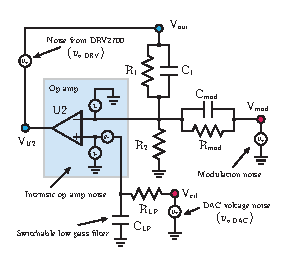
\includegraphics[width=\columnwidth]{fig/NoiseModel.ai}
\caption{Noise model. \label{Fig:NoiseModel}}
\end{figure}

We analyze the noise performance of the circuit according to the model shown in Figure~\ref{Fig:NoiseModel}, where noise spectral densities are calculated at the node HV.
Here, we consider contributions from the intrinsic op-amp noise, the DAC (injected at the node $V_{\text{DC}}$), Johnson-Nyquist noise of the passive components, and any additional noise injected at the modulation input node $V_{\text{mod}}$.
We also discuss, given our choice of op-amp, the noise rejection ratio from the DRV2700 flyback regulator.

First, the noise gain ($NG$) for this amplifier configuration is given by
\begin{align}
\label{Eq:NG}
%NG(s) &= 1 + \frac{R_1 \epar C_1}{R_2 \epar \left(R_{\text{mod}} \epar C_{\text{mod}}\right)}
%NG(s) &= 1 + \frac{R_1~||~C_1}{R_2R_{\text{mod}} C_{\text{mod}}}
NG(s) &= 1 + \frac{Z_1}{R_2 \epar Z_{\text{mod}}}
\end{align}
where we've defined the equivalent impedances $Z_1 = R_1/(1+R_1 C_1 s)$ and $Z_{\text{mod}} = R_{\text{mod}}/(1+R_{\text{mod}} C_{\text{mod}} s)$, and $s = i\omega$ is the frequency in the Laplace domain.
By design, we've chosen $Z_1 \equiv Z_{\text{mod}}$ such that the signal gain from the node $V_{\text{mod}}$ is unity.
This reduces Eq.~(\ref{Eq:NG}) to
\begin{align}
\label{Eq:RedNG}
NG(s) &= 2 + \frac{Z_1}{R_2}
\end{align}

The op-amp noise is parametrized by two noise contributions -- $e_n$, the input voltage noise power spectral density (PSD), and $i_n$, the input current noise PSD. 
For the LM7171, $e_n = \SI[per-mode=symbol]{14}{\nano\volt\per\sqrthz}$ and $i_n = \SI[per-mode=symbol]{1.5}{\pico\ampere\per\sqrthz}$ at $\SI{10}{\kilo\hertz}$.
The voltage noise is summed in at the non-inverting input, while the current noise is present at both inputs.
To convert $i_n$ to an equivalent voltage noise $e_n$, we multiply by the impedances $Z_n$, $Z_p$ seen by the inverting and non-inverting nodes, respectively.
These are calculated as
\begin{align}
\begin{split}
\label{Eq:ZnZp}
Z_n &= Z_1 \epar Z_{\text{mod}} \epar  R_2   = \frac{Z_1}{2} \epar R_2 \\
Z_p &= R_{\text{LP}}  \big|\big|\frac{1}{s~C_{\text{LP}}}
\end{split}
\end{align}
The total noise contribution of the op-amp (referenced to the output) is
\begin{align}
\label{Eq:OpAmpNoise}
e_{n,\text{op-amp}} &= NG(s)\sqrt{e_n^2 + (Z_n i_n)^2 + (Z_p i_n)^2}
\end{align}

We now calculate the noise contribution of the DAC. 
The noise signal gain from the node $V_{\text{DC}}$ is given by
\begin{align}
\begin{split}
\label{Eq:Gdc}
G_{\text{DC}} &= \left(\frac{1}{1+sR_{\text{LP}}C_{\text{LP}}}\right)\left(1+\frac{Z_1}{R_2\epar Z_{\text{mod}}}\right) \\
&= \left(\frac{1}{1+sR_{\text{LP}}C_{\text{LP}}}\right)NG(s)
\end{split}
\end{align}
Thus, the DAC voltage noise contribution is just $e_{n,\text{DAC}} = G_{\text{DC}} v_{n,\text{DAC}}$. The AD5663 has a white noise floor of \SI[per-mode=symbol]{100}{\nano\volt\per\sqrthz} (\SI{1}{\kilo\hertz} corner frequency).
For our circuit, this is the dominant noise contribution.
Each noise source is shown and tabulated in Table~\ref{Tab:noise}.


\begin{table}
\caption{Various noise contributions. -- should we just tabulate RMS?}
\label{Tab:noise}
\begin{ruledtabular}
\centering
\begin{tabular}{lcc}
 \multirow{2}{*}{Noise source} & \multicolumn{2}{c}{Voltage PSD (\si[per-mode=symbol]{\nano\volt\per\sqrthz})} \\ \cline{2-3}
\rule{0pt}{3ex} & (input-referred) & (output-referred) \\ 
\hline
$e_n$ (op-amp) & \SI{14} (white); \SI{30} ($1/f$)  & \\
$i_n$ (op-amp) &    & \\
DAC &    & \\
Johnson-Nyquist & & \\ \hline
\textbf{total} & &
\end{tabular}
\end{ruledtabular}
\end{table}



\section{Results}
\label{Sec:Results}
Noise analysis, bandwidth, (DC) stability, etc.

We characterized the performance of the high-voltage piezo driver with a few different metrics.
In Fig.~XX, you can see the noise power spectral density.
This trace was taken on an SRSXXX spectrum analyzer, AC coupled to the high-voltage output with a \SI{0.5}{\hertz} high-pass filter circuit shown in Fig.~XX(b).

\begin{itemize}
\item $1/f \rightarrow$ white noise corner frequency
\item white noise spectral density
\item RMS noise (0.1 - 10 Hz; 10 Hz - 10 kHz, or something similar) -- use SRS voltage preamp?
\item How effective is the LM7171 at reducing switching noise? look at FFT power before final filter resistor, and at output of op amp (dBc spec)
\item compare noise to predicted values
\item longterm trace on kiethly -- across voltage divider at output? Monitor vs temperature? -- need to find low Tc resistors, at least.
\item see what dependence is on power source -- eg, JQI power supply vs lab supply vs very quiet voltage regulator?
\item current draw -- display in some ``bottom line'' specs table?
\item bandwidth measurements -- full scale triangle ramp, small signal bandwidth -- discuss limitations on this (eg, also versus different piezo loads)
\item Lock a laser, show RMS noise fluct vs. old piezo?
\item compare to SC100 toptica controller? even if just internally.
\end{itemize}

\section{Conclusion}
\label{Sec:Conclusion}


% If in two-column mode, this environment will change to single-column format so that long equations can be displayed. 
% Use only when necessary.
%\begin{widetext}
%$$\mbox{put long equation here}$$
%\end{widetext}

% Figures should be put into the text as floats. 
% Use the graphics or graphicx packages (distributed with LaTeX2e). EPSFig is no longer fully supported.
% See the LaTeX Graphics Companion by Michel Goosens, Sebastian Rahtz, and Frank Mittelbach for examples. 
%
% Here is an example of the general form of a figure:
% Fill in the caption in the braces of the \caption{} command. 
% Put the label that you will use with \ref{} command in the braces of the \label{} command.
%
% \begin{figure}
% \includegraphics{}% % Important NOTE: Please make certain your figures do not include local directory paths. ex. "c:\file\sub\fig1.eps"
% \caption{\label{}}%
% \end{figure}

% Tables may be be put in the text as floats.
% Here is an example of the general form of a table:
% Fill in the caption in the braces of the \caption{} command. Put the label
% that you will use with \ref{} command in the braces of the \label{} command.
% Insert the column specifiers (l, r, c, d, etc.) in the empty braces of the
% \begin{tabular}{} command.
%
% \begin{table}
% \caption{\label{} }
% \begin{tabular}{}
% \end{tabular}
% \end{table}

% If you have acknowledgments, this puts in the proper section head.
%\begin{acknowledgments}
% Put your acknowledgments here.
%\end{acknowledgments}

% Create the reference section using BibTeX:
%\bibliography{your-bib-file}
% Run this once to generate your BBL file. Then copy the contents of your BBL file into your main latex file, commenting out "\bibliography"

\end{document}
%
% ****** End of file aiptemplate.tex ******
